\documentclass{article}

\usepackage{cite}
\usepackage{amsmath,amssymb,amsfonts}
\usepackage{algorithmic}
\usepackage{graphicx}
\usepackage{textcomp}
\usepackage{xcolor}
\usepackage{url}
\usepackage{tikz}
\usetikzlibrary{positioning,arrows.meta}
\usepackage[
    left=3cm,
    right=3cm,
    top=2cm,
    bottom=2cm
]{geometry}

\setlength{\parskip}{0.4em}

\begin{document}
\title{ATAI Evaluation Event II\\[0.3em]
\large \textit{AGENT\_ACCOUNT\_NAME}}

\author{
Georgios Stratidis (\textit{USER\_ACCOUNT\_NAME})
\and
TEAMMATE\_FULL\_NAME (\textit{USER\_ACCOUNT\_NAME})
}

\date{}

\maketitle
\noindent
\textbf{Max. 2 pages.} Additional pages will not be read.
References and screenshots are excluded from the page limit.

\section{Agent Overview and Capabilities}

Our agent answers single-hop factual questions about movies from the provided knowledge graph, which is derived from Wikidata~\cite{vrandecic2014wikidata}. Every natural-language question is turned into a SPARQL query~\cite{harris2013sparql}, and the answer is read from the graph and returned as a template sentence, e.g.\ ``\textit{The factual answer is: Jeong Seo-kyeong and Park Chan-wook}''. Several answers are joined with ``and''. The agent handles both directions of a triple: the property of a movie (``\textit{Who directed Alien?}'') and the movies of a person (``\textit{Which movies did Sofia Coppola direct?}''). It also answers counts (``\textit{How many movies has Céline Sciamma directed?}'') and the earliest or latest film of a person, as in the official example about Sofia Coppola. Titles may be quoted or unquoted, in lower case, or contain typos. When the agent cannot find the entity, the property, or the fact, it says so instead of guessing. Raw SPARQL queries from Evaluation I are still executed directly. The agent serves several chatrooms in parallel and keeps running when single requests fail.

\section{Adopted Methods}

\begin{itemize}
    \item \textbf{Knowledge graph store.} We load \texttt{graph.nt} (2.4M triples) once into an on-disk store of pyoxigraph\footnote{\url{https://pyoxigraph.readthedocs.io/}}, a SPARQL~1.1 engine written in Rust. Building takes 11\,s; afterwards the store opens in 0.01\,s, and queries run outside Python's global interpreter lock, so requests from several chatrooms are answered in parallel.
    \item \textbf{Entity linking.} As in tutorial 04a, we build label dictionaries at startup (\texttt{ent2lbl}, \texttt{lbl2ent}; 123k labels, 5\,s). A quoted title is looked up directly; otherwise we search for the longest word sequence that is a label, preferring capitalised spans. For typos we fall back to fuzzy matching with RapidFuzz\footnote{\url{https://github.com/rapidfuzz/RapidFuzz}} using the optimal string alignment distance~\cite{damerau1964technique} (similarity $\geq 0.85$), which counts a swap or substitution (``Godfahter'') as a single edit.
    \item \textbf{Relation linking.} The question is matched against the graph's own property labels (497, e.g.\ ``director'', ``box office'') plus a small data file of everyday wordings for 26 common properties (``directed'', ``starred'', ``came out''). The longest matching phrase is tried first.
    \item \textbf{Query construction.} Four SPARQL templates: lookup, count, earliest/latest film by release date, and an \texttt{ASK} query that checks whether a fact exists.
    \item \textbf{Platform.} Speakeasy's Python client (speakeasypy) and Python's thread pools for concurrency.
\end{itemize}

\section{Pipeline}

Figure~\ref{fig:pipeline} shows the pipeline. Given the question ``\textit{Who is the director of Good Will Hunting?}'', the agent first checks whether the message is a SPARQL query; it is not, so it is treated as a factual question. Entity linking finds the longest capitalised word sequence that is a graph label, ``Good Will Hunting'', which maps to a single entity, \texttt{wd:Q193835} (a film). Relation linking finds the phrase ``director'', the label of \texttt{wdt:P57}. Two \texttt{ASK} queries determine the direction: the film has a director, but it is not itself the director of anything, so the answer is the object of the triple. The agent then runs
\begin{center}
\texttt{SELECT DISTINCT ?x ?label WHERE \{ wd:Q193835 wdt:P57 ?x .}\\
\texttt{OPTIONAL \{ ?x rdfs:label ?label \} \} LIMIT 200}
\end{center}
and verbalises the labels of the results: ``\textit{The factual answer is: Gus Van Sant}''. The answer is correct. The whole request takes under 10\,ms.

When a label is ambiguous, the same pipeline decides: four entities are called ``The Godfather'' (a film, a novel, a film trilogy and a video game). Candidates are ordered films first, then by the number of triples, and the first candidate that actually has the asked property in the graph is used. For ``\textit{Who directed The Godfather?}'' this is the 1972 film, and the answer is ``Francis Ford Coppola''.

\section{Improvements}

\textbf{Faster and parallel graph access.} Our first agent parsed the 290\,MB graph with rdflib at every start and answered messages one at a time, so one slow query blocked all chatrooms. Switching to a persistent pyoxigraph store reduced the start-up to a few seconds, and a worker pool with one lock per chatroom answers different rooms in parallel while keeping the order within a room. Median answer time is now below 10\,ms, and slow requests get a polite fallback reply after a timeout.

\textbf{More precise entity linking.} Early versions matched lower-case phrases as titles, e.g.\ ``\textit{What is the box office of Interstellar?}'' was linked to the film \textit{The Box}. We now prefer capitalised spans. When only part of a longer capitalised title is a known label (``\textit{Don't Look Up}'', which is not in the graph, contains the film \textit{Up}), the agent answers that it does not know the movie instead of answering for the fragment.

\textbf{Simplification.} We removed rule-based features that belong to later evaluations (negation, yes/no questions, follow-ups); the agent is now about 1,100 lines of Python, and the remaining behaviour is easier to test. A regression set of 57 questions with expected answers obtained from hand-written SPARQL queries passes completely.

\section{Additional Features}

\begin{itemize}
    \item \textbf{SPARQL pass-through} (Evaluation I): queries with or without \texttt{PREFIX} lines, also wrapped in \texttt{'''} or code fences, are executed directly.
    \item \textbf{Robustness:} timeouts for queries (20\,s) and replies (25\,s), fallback replies on errors, automatic re-login with exponential back-off, and a heartbeat in the log.
    \item \textbf{Testing:} an offline command-line interface that prints each pipeline step, 74 unit tests on small fixture graphs, and the 57-question regression set; all pass on Python~3.13, the version used on Nuvolos.
\end{itemize}

\begin{figure}[p]
    \centering
    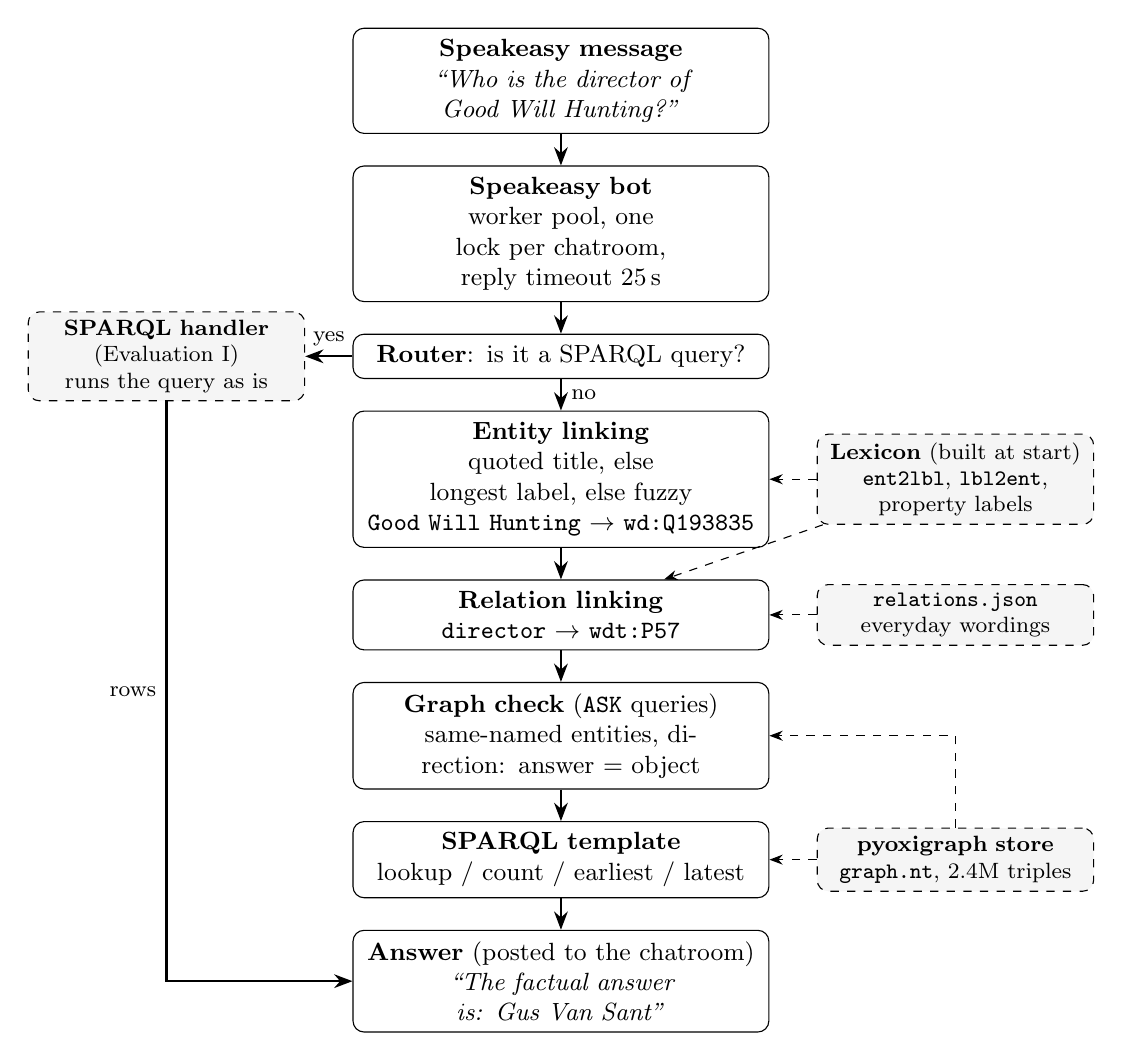
\begin{tikzpicture}[
    node distance=4mm and 6mm,
    box/.style={draw, rounded corners, align=center, font=\small, text width=5cm, inner sep=4pt},
    side/.style={draw, dashed, rounded corners, align=center, font=\footnotesize, text width=3.3cm,
                 inner sep=3pt, fill=gray!8},
    arr/.style={-{Stealth}, thick},
    use/.style={-{Stealth}, dashed}
]
    % main flow
    \node[box] (msg) {\textbf{Speakeasy message}\\ \textit{``Who is the director of Good Will Hunting?''}};
    \node[box, below=of msg] (bot) {\textbf{Speakeasy bot}\\ worker pool, one lock per chatroom,\\ reply timeout 25\,s};
    \node[box, below=of bot] (route) {\textbf{Router}: is it a SPARQL query?};
    \node[box, below=of route] (entity) {\textbf{Entity linking}\\ quoted title, else longest label, else fuzzy\\
        \texttt{Good Will Hunting} $\rightarrow$ \texttt{wd:Q193835}};
    \node[box, below=of entity] (relation) {\textbf{Relation linking}\\ \texttt{director} $\rightarrow$ \texttt{wdt:P57}};
    \node[box, below=of relation] (check) {\textbf{Graph check} (\texttt{ASK} queries)\\
        same-named entities, direction: answer = object};
    \node[box, below=of check] (query) {\textbf{SPARQL template}\\ lookup / count / earliest / latest};
    \node[box, below=of query] (answer) {\textbf{Answer} (posted to the chatroom)\\
        \textit{``The factual answer is: Gus Van Sant''}};

    % resources
    \node[side, right=of entity] (lex) {\textbf{Lexicon} (built at start)\\ \texttt{ent2lbl}, \texttt{lbl2ent},\\ property labels};
    \node[side, right=of relation] (syn) {\texttt{relations.json}\\ everyday wordings};
    \node[side, right=of query] (store) {\textbf{pyoxigraph store}\\ \texttt{graph.nt}, 2.4M triples};
    \node[side, left=of route] (sparql) {\textbf{SPARQL handler}\\ (Evaluation I)\\ runs the query as is};

    % edges
    \draw[arr] (msg) -- (bot);
    \draw[arr] (bot) -- (route);
    \draw[arr] (route) -- node[right, font=\footnotesize] {no} (entity);
    \draw[arr] (route) -- node[above, font=\footnotesize] {yes} (sparql);
    \draw[arr] (entity) -- (relation);
    \draw[arr] (relation) -- (check);
    \draw[arr] (check) -- (query);
    \draw[arr] (query) -- (answer);
    \draw[arr] (sparql.south) |- node[pos=0.25, left, font=\footnotesize] {rows} (answer.west);
    \draw[use] (lex) -- (entity);
    \draw[use] (lex) -- (relation);
    \draw[use] (syn) -- (relation);
    \draw[use] (store) -- (query);
    \draw[use] (store) |- (check);
\end{tikzpicture}

    \caption{Pipeline of our agent for Evaluation II, with the intermediate results for the example question.
    Dashed boxes are resources built once at start-up; dashed arrows show where they are used.}
    \label{fig:pipeline}
\end{figure}

\bibliographystyle{abbrv}
\bibliography{references}

\end{document}
